\documentclass[tikz,border=10pt]{standalone}
\usepackage{amsmath}
\usetikzlibrary{positioning, arrows.meta, calc}

% Define colors
\definecolor{transblue}{RGB}{70,130,180}
\definecolor{transorange}{RGB}{255,140,0}
\definecolor{transgreen}{RGB}{50,205,50}

\begin{document}

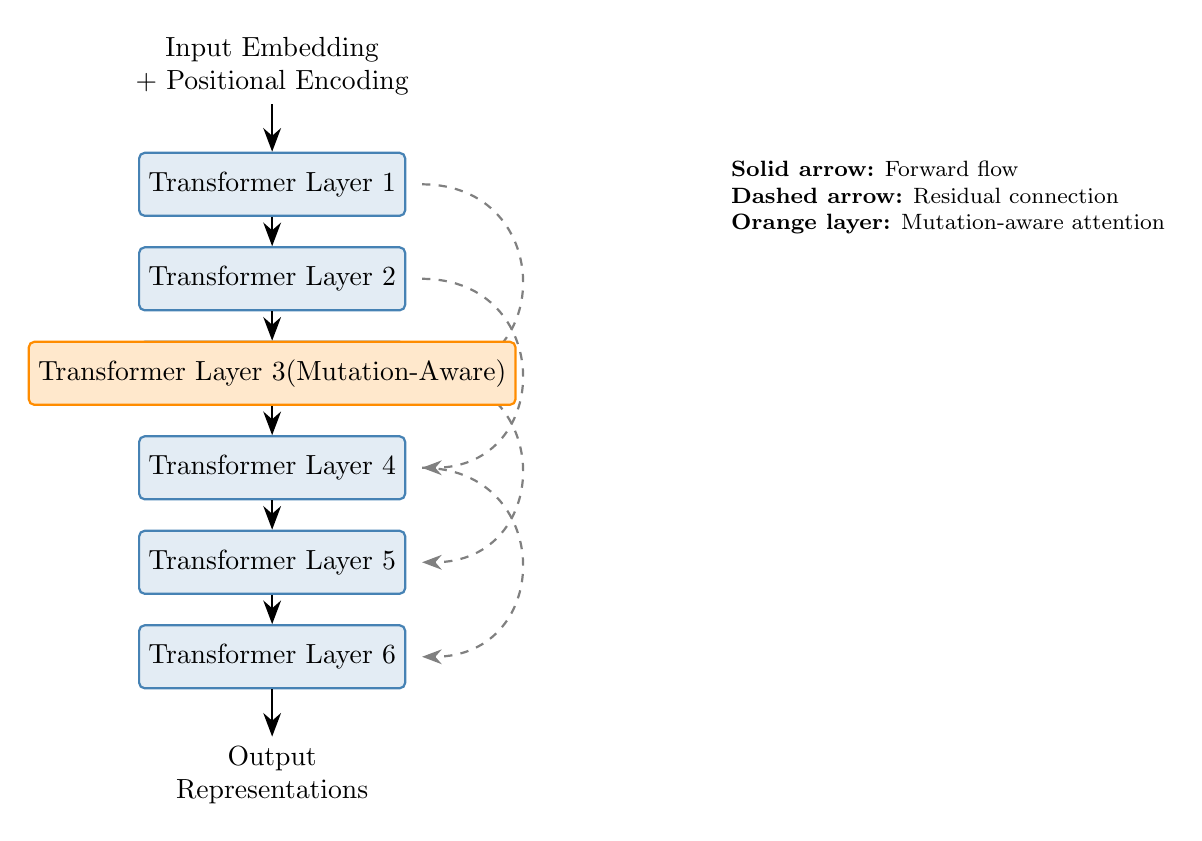
\begin{tikzpicture}[
    layer/.style={rectangle, draw=transblue, fill=transblue!15, thick, minimum width=3cm, minimum height=0.8cm, rounded corners=2pt},
    arrow/.style={-{Stealth[length=3mm]}, thick},
    residual/.style={-{Stealth[length=2.5mm]}, dashed, gray, thick}
]

% Parameters
\def\nLayers{6}
\def\layerSpacing{1.2}

% Draw stacked layers
\foreach \i in {1,...,\nLayers} {
    \node[layer] (L\i) at (0, {-(\i-1)*\layerSpacing}) {Transformer Layer \i};
}

% Input and output
\node[above=0.6cm of L1, align=center] (input) {Input Embedding \\ + Positional Encoding};
\node[below=0.6cm of L\nLayers, align=center] (output) {Output \\ Representations};

% Arrows between layers
\draw[arrow] (input) -- (L1);
\foreach \i [evaluate=\i as \next using int(\i+1)] in {1,...,\numexpr\nLayers-1\relax} {
    \draw[arrow] (L\i) -- (L\next);
}
\draw[arrow] (L\nLayers) -- (output);

% Residual connections (skip connections)
\foreach \i [evaluate=\i as \next using int(\i+2)] in {1,...,\numexpr\nLayers-2\relax} {
    \draw[residual] ($(L\i.east)+(0.2,0)$) to[out=0,in=0,looseness=1.8] ($(L\next.east)+(0.2,0)$);
}

% Optional: highlight one layer (e.g., mutation-aware attention)
\node[layer, draw=transorange, fill=transorange!20, thick] at (L3) {Transformer Layer 3 \\ (Mutation-Aware)};

% Legend
\node[anchor=north west, align=left, font=\footnotesize] at ([xshift=4cm]L1.north east) {
    \textbf{Solid arrow:} Forward flow \\
    \textbf{Dashed arrow:} Residual connection \\
    \textbf{Orange layer:} Mutation-aware attention
};

\end{tikzpicture}

\end{document}
